\documentclass[12pt]{article}
\usepackage[utf8]{inputenc}
\usepackage{geometry}
\geometry{letterpaper, margin=0.25in}
\usepackage{graphicx} 
\usepackage{parskip}
\usepackage{booktabs}
\usepackage{array} 
\usepackage{paralist} 
\usepackage{verbatim}
\usepackage{subfig}
\usepackage{fancyhdr}
\usepackage{sectsty}
\usepackage[shortlabels]{enumitem}

\pagestyle{fancy}
\renewcommand{\headrulewidth}{0pt} 
\lhead{}\chead{}\rhead{}
\lfoot{}\cfoot{\thepage}\rfoot{}

%%% ToC (table of contents) APPEARANCE
\usepackage[nottoc,notlof,notlot]{tocbibind} 
\usepackage[titles,subfigure]{tocloft}
\renewcommand{\cftsecfont}{\rmfamily\mdseries\upshape}
\renewcommand{\cftsecpagefont}{\rmfamily\mdseries\upshape} %

\usepackage{amsmath}
\usepackage{amssymb}
\usepackage{mathtools}
\usepackage{empheq}
\usepackage{xcolor}
\usepackage{bbm}
\usepackage{tikz}
\usepackage{pgfplots}
\usepackage{tikz-cd}
\pgfplotsset{compat=1.18}

\newcommand{\ans}[1]{\boxed{\text{#1}}}
\newcommand{\vecs}[1]{\langle #1\rangle}
\renewcommand{\hat}[1]{\widehat{#1}}

\renewcommand{\P}{\mathbb{P}}
\newcommand{\R}{\mathbb{R}}
\newcommand{\E}{\mathbb{E}}
\newcommand{\Z}{\mathbb{Z}}
\newcommand{\N}{\mathbb{N}}
\newcommand{\Q}{\mathbb{Q}}
\newcommand{\C}{\mathbb{C}}

\newcommand{\ind}{\mathbbm{1}}
\newcommand{\qed}{\quad \blacksquare}

\newcommand{\brak}[1]{\left\langle #1 \right\rangle}
\newcommand{\bra}[1]{\left\langle #1 \right\vert}
\newcommand{\ket}[1]{\left\vert #1 \right\rangle}

\newcommand{\abs}[1]{\left\vert #1 \right\vert}
\newcommand{\mfX}{\mathfrak{X}}
\newcommand{\ep}{\varepsilon}

\newcommand{\Ec}{\mathcal{E}}
\newcommand{\A}{\mathcal{A}}
\newcommand{\F}{\mathcal{F}}
\newcommand{\Cc}{\mathcal{C}}
\newcommand{\B}{\mathcal{B}}
\newcommand{\M}{\mathcal{M}}
\newcommand{\X}{\chi}
\renewcommand{\L}{\mathcal{L}}

\newcommand{\sub}{\subseteq}
\newcommand{\st}{\text{ s.t. }}
\newcommand{\card}{\text{card }}
\renewcommand{\div}{\vspace*{10pt}\hrule\vspace*{10pt}}
\newcommand{\surj}{\twoheadrightarrow}
\newcommand{\inj}{\hookrightarrow}
\newcommand{\biject}{\hookrightarrow \hspace{-8pt} \rightarrow}
\renewcommand{\bar}[1]{\overline{#1}}
\newcommand{\overcirc}[1]{\overset{\circ}{#1}}
\newcommand{\diam}{\text{diam }}

\renewcommand{\Re}{\text{Re}\,}
\renewcommand{\Im}{\text{Im}\,}
\newcommand{\sign}{\text{sign}\,}

\newcommand*{\tbf}[1]{\ifmmode\mathbf{#1}\else\textbf{#1}\fi}

\usepackage{tcolorbox}
\tcbuselibrary{breakable, skins}
\tcbset{enhanced}
\newenvironment*{tbox}[2][gray]{
    \begin{tcolorbox}[
        parbox=false,
        colback=#1!5!white,
        colframe=#1!75!black,
        breakable,
        title={#2}
    ]}
    {\end{tcolorbox}}

\newenvironment*{exercise}[1][red]{
    \begin{tcolorbox}[
        parbox=false,
        colback=#1!5!white,
        colframe=#1!75!black,
        breakable
    ]}
    {\end{tcolorbox}}

\newenvironment*{proof}[1][blue]{
\begin{tcolorbox}[
    parbox=false,
    colback=#1!5!white,
    colframe=#1!75!black,
    breakable
]}
{\end{tcolorbox}}

\title{APMA 1360: Homework 3}
\author{Milan Capoor}
\date{14 February 2025}

\begin{document}
\maketitle

\section{(5 points) Classifying Bifurcation diagrams}
Consider the following three potential bifurcation diagrams for a differential equation $\dot{x}=f(x,\mu)$ on the line, where stable and unstable equilibria are drawn as solid and dashed curves, respectively. For each diagram, circle all bifurcation points in the $(\mu,x)$-plane and classify them as saddle-node, transcritical, and pitchfork, or argue why the resulting diagram is impossible.
\begin{center}
    \begin{tikzpicture}
        \node at (0, 0) {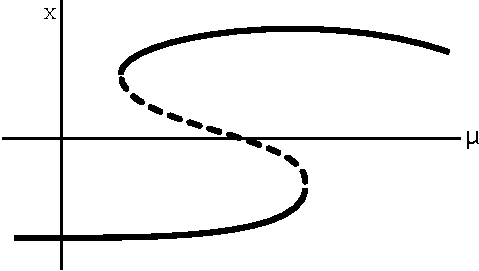
\includegraphics[scale=0.7]{Images/Assignment_Figure_2.pdf}};

        \node[scale=1.5, red] at (-1.4, 0.7) {$\bullet$};
        \node[scale=1.5, red] at (0.8, -0.7) {$\bullet$};

        \node at (6, 0) {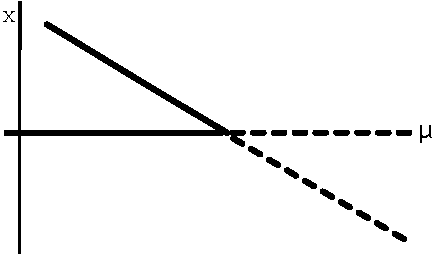
\includegraphics[scale=0.7]{Images/Assignment_Figure_3.pdf}};

        \node[scale=1.5, green] at (6.1, -0.1) {$\bullet$};

        \node at (12, 0) {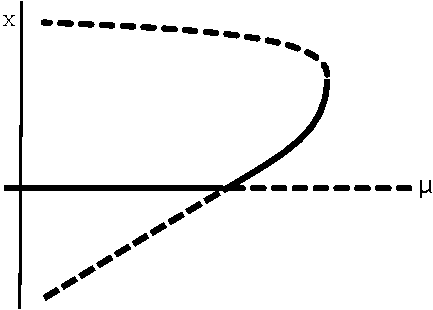
\includegraphics[scale=0.7]{Images/Assignment_Figure_4.pdf}};

        \node[scale=1.5, green] at (12.1, -0.4) {$\bullet$};
        \node[scale=1.5, red] at (13.3, 0.9) {$\bullet$};

        \node[red, scale=2] (r) at (3, -3) {$\bullet$};
        \node[green, scale=2] (g) at (3, -4) {$\bullet$};
        \node[xshift=1.7cm] at (r) {Saddle-node};
        \node[xshift=1.7cm] at (g) {Transcritical};


    \end{tikzpicture}
\end{center}

\color{blue}
However, the second diagram is not possible. Let $(\mu_*, u_*)$ be the hypothetical transcritical equilibrium. To have two stable equilibria for $\mu < \mu_*$, we would need solutions to move up to the $u = -O(\mu)$ curve and down to the $u = 0$ curve. But this suggests the existence of an unstable equilibrium between the two stable equilibria, which is not possible in the given diagram.
\color{black}

\pagebreak

%%%%%%%%%%%%%%%%%%%%%%%%%%%%%%%%

\section{(5 points) Which bifurcations do we expect to encounter?}

Consider the differential equation $\dot{u}=f(u,\mu)$. For each of the different functions listed below, argue whether and why, or why not, you expect to see a saddle-node, pitchfork or transcritical bifurcation to occur at $u=0$ for some value of $\mu$.
\begin{enumerate}[(i)]
    \item $f(u,\mu) = \mu-3u^2$

          \color{blue}
          \begin{enumerate}
              \item  $f(0, \mu) = \mu \neq 0$ so we cannot see a transcritical bifurcation.
              \item $f(u, \mu)$ is even in $u$ so we cannot see a pitchfork bifurcation.
              \item Since we are quadratic in the $\mu$-$u$ plane, we expect to see a saddle-node bifurcation.
          \end{enumerate}
          \color{black}

    \item $f(u,\mu) = \mu u+u\sin u$

          \color{blue}
          \begin{enumerate}
              \item   $f(0, \mu) = 0 \quad \forall \mu$ so a transcritical bifurcation is likely.
              \item $f(-u, \mu) = -\mu u - u(\sin(-u)) = -\mu u + u \sin u \neq f(u, \mu)$ so we are again not odd in $u$ and cannot see a pitchfork bifurcation.
              \item $f_u = \mu + \sin u + u\cos u \implies f_{uu} = 2\cos u - u \sin u \neq 0$ and $f_{\mu} = u \neq 0$ so a saddle-node bifurcation is possible.
          \end{enumerate}
          \color{black}

    \item $f(u,\mu) = \mu u - u^2\sin u + u^5$

          \color{blue}
          \begin{enumerate}
              \item $f(0, \mu) = \mu \neq 0$ so we cannot see a transcritical bifurcation.
              \item $f(u, \mu)$ is odd in $u$ so we could see a pitchfork bifurcation.
              \item $f_{uu} = -2\sin u - 2u\cos u + 20u^3 \neq 0$ and $f_{\mu} = u \neq 0$ so a saddle-node bifurcation is possible.
          \end{enumerate}
          \color{black}

\end{enumerate}
\emph{Note:} you do \textbf{not} need to find bifurcation points or analyse them. It suffices to state which bifurcations you expect to find, which you think cannot occur, and provide arguments that support your statements. In other words, the point of this problem is not to find all bifurcation point explicitly by solving these equations but rather to exclude certain bifurcations, because they should not occur and argue why not.


\pagebreak

%%%%%%%%%%%%%%%%%%%%%%%%%%%%%%%%

\section{(5 points) Singular perturbations and the implicit function theorem}

This problem will explore the reasons for why we may be able to drop the second-order derivative term in the model of the bead on the rotating hoop. Consider the differential equation
\begin{equation}\label{e1}
    \epsilon \frac{d^2 u}{dt^2} + \frac{d u}{d t} + u = 0.
\end{equation}
\begin{enumerate}[(i)]
    \item Show that $u(t)=u_0e^{-t}$ is the general solution of the equation $\dot{u}+u=0$, that is (\ref{e1}) with $\epsilon=0$.

          \color{blue}
          Let $u(t) = u_0 e^{-t}$. Then $\dot u = -u_0 e^{-t}$ so
          \[\dot u + u = -u_0 e^{-t} + u_0 e^{-t} = 0\]
          so $u(t)$ is a solution of the equation $\dot u + u = 0$.
          \color{black}

    \item Show that $u(t)=u_1e^{\lambda t}$ is a solution of (\ref{e1}) for each value of $u_1$ if, and only if, $\epsilon\lambda^2+\lambda+1=0$.

          \color{blue}
          $(\implies)$ If $u_1 e^{\lambda t}$ is a solution, then
          \begin{align*}
              \ep u_1 \lambda^2 e^{\lambda t} + u_1 \lambda e^{\lambda t} + u_1 e^{\lambda t} = 0 \\
              \implies u_1 e^{\lambda t} (\ep \lambda^2 + \lambda + 1) = 0
          \end{align*}

          For $u_1 \neq 0$, $u_1 e^{\lambda t} \neq 0$ so we must have $\ep \lambda^2 + \lambda + 1 = 0$.

          $(\impliedby)$ Let $\ep \lambda^2 + \lambda + 1 =0$. Then
          \[\ep \frac{d^2 u}{dt^2} + \frac{d u}{d t} + u = u_1 e^{\lambda t} (\ep \lambda^2 + \lambda + 1) = 0\]
          hence $u(t) = u_1 e^{\lambda t}$ is a solution of (\ref{e1}).
          \color{black}

    \item Use the implicit function theorem to prove that there is a solution of the form $u(t)=u_1 e^{\lambda_1(\epsilon)t}$ where $\lambda_1(\epsilon)=-1+O(\epsilon)$ is $C^\infty$.

          \color{blue}
          In (ii), we showed that $u(t) = u_1 e^{\lambda t}$ is a solution of (\ref{e1}) iff $\ep \lambda^2 + \lambda + 1 = 0$.

          Hence, let $f(\lambda, \ep) = \ep \lambda^2 + \lambda + 1$.

          Then $f(-1, 0) =0$ and $f_{\lambda}(-1, 0) = 1 \neq 0$ so we may apply the IFT in a neighborhood of $(-1, 0)$.

          In particular, this means there is a $C^{\infty}$ function $\lambda_1(\ep)$ such that $f(\lambda_1(\ep), \ep) = 0$ and $\lambda_1(0) = -1$. In the Taylor expansion, $\lambda_1(\ep) = -1 + O(\ep)$.

          Hence, $\ep \lambda_1(\ep)^2 + \lambda_1(\ep) + 1 = 0 \implies u(t) = u_1 e^{\lambda_1(\ep)t}$ is a solution.

          \color{black}

    \item Show that for each $\varepsilon>0$ there is a second solution of the form $u(t)=u_2e^{\lambda_2(\epsilon)t/\epsilon}$ for arbitrary $u_2$ where $\lambda_2(\epsilon)=-1+O(\epsilon)$ is $C^\infty$. \emph{Hint:} substitute $\lambda=x/\epsilon$ into the equation $\epsilon\lambda^2+\lambda+1=0$ and use the implicit function theorem.

          \color{blue}
          Let $\ep > 0$. Again, we search for solutions to $\ep \lambda^2 + \lambda + 1 = 0$.

          Let $\lambda = \frac{x}{\ep}$ so
          \[\ep \left(\frac{x}{\ep}\right)^2 + \frac{x}{\ep} + 1 = 0 \implies x^2 + x + \ep = 0\]

          In particular, this means that solutions to $u(t) = u_2 e^{\lambda t}$ correspond to solutions of
          \[f(x, \ep) = x^2 + x + \ep = 0\]

          Notice that $f(0, 0) = 0$ and $f_x(0, 0) = 1 \neq 0$ so we may apply the IFT in a neighborhood of $(0, 0)$. Hence, $\exists \lambda_2(\ep) \in C^{\infty}$ such that $f(\lambda_2(\ep), \ep) = 0$ and $\lambda_2(0) = 0$. Again taking a Taylor expansion, $\lambda_2(\ep) = -1 + O(\ep)$.

          Above, we defined $\lambda = \frac{x}{\ep}$ so that means
          \[u(t) = u_2 e^{\lambda_2(\ep)t/\ep}\]
          is a solution of (\ref{e1}) with $\lambda_2(\ep) = -1 + O(\ep)$.

          \color{black}

    \item Use these results to write down the general solution of (\ref{e1}) and compare its behavior with that of the differential equation $\dot{u}+u=0$ for $0<\epsilon\ll1$.

          \color{blue}
          The general solution of (\ref{e1}) is given by ,
          \[u(t) = u_1 e^{\lambda_1(\ep)t} + u_2 e^{\lambda_2(\ep)t/\ep} \]
          where $\lambda_1(\ep) = -1 + O(\ep)$ and $\lambda_2(\ep) = -1 + O(\ep)$.

          Intuitively, we should have that for $\ep \approx 0$, the solution to $\ep\ddot u + \dot u + u =0$ should behave like the solution to $\dot u + u = 0$.

          We can check: For $0< \ep \ll 1$, we have $\lambda_1(\ep) \approx -1$ and $\lambda_2(\ep) \approx -1$ so
          \[u(t) = u_1 e^{-t + tO(\ep)} + u_2e^{-\frac{t}{\ep} + \frac{O(\ep)}{\ep} t} \approx u_1e^{-t} + u_2 \approx u_1e^{-t}\]
          as expected!
          \color{black}

\end{enumerate}

%%%%%%%%%%%%%%%%%%%%%%%%%%%%%%%%

\end{document}
